\documentclass[a4paper]{article}
\usepackage[a4paper,margin=0mm]{geometry}
\usepackage{fontspec}
\usepackage{unicode-math}
\usepackage{tikz}
\usetikzlibrary{fit,calc,positioning}
\usepackage[table]{xcolor}
\usepackage[absolute]{textpos}
\usepackage{array}

\setmainfont{Libertinus Serif}
\setsansfont{Libertinus Sans}
\setmathfont{Libertinus Math}

\definecolor{accent}{HTML}{F46530}
\definecolor{badge}{HTML}{FFBDA5}
\definecolor{ink}{HTML}{2A2E30}

\setlength{\TPHorizModule}{1mm}
\setlength{\TPVertModule}{1mm}
\setlength{\parindent}{0pt}
\pagestyle{empty}

\newcommand{\topicheader}[2]{%
\begin{textblock*}{194mm}(16mm,10mm)
\begin{tikzpicture}
\node[fill=accent,text=white,font=\sffamily\bfseries\fontsize{13}{13}\selectfont,
      minimum width=9mm,minimum height=9mm,inner sep=0pt] at (4.5mm,-4.5mm) {#1};
\node[font=\sffamily\bfseries\fontsize{15}{16}\selectfont,text=ink,anchor=west] at (12mm,-4.5mm) {#2};
\end{tikzpicture}
\end{textblock*}
\begin{textblock*}{194mm}(16mm,22.5mm)

\begin{tikzpicture}
\fill[accent] (0,0) rectangle (194mm,0.5mm);
\end{tikzpicture}
\end{textblock*}
}

\newcommand{\pagekicker}[1]{%
\begin{textblock*}{100mm}(16mm,25.5mm)
\begin{tikzpicture}
\node[fill=ink,text=white,font=\sffamily\bfseries\fontsize{8}{8}\selectfont,
      inner sep=2.2pt,rounded corners=1pt] {\MakeUppercase{#1}};
\end{tikzpicture}
\end{textblock*}
}

\newcommand{\pagefooter}[1]{%
\begin{textblock*}{194mm}(8mm,286.41mm)
  
\begin{tikzpicture}
    \fill[accent] (0,0) rectangle (194mm,0.6mm);
  \end{tikzpicture}
\end{textblock*}
\begin{textblock*}{63.59mm}(8mm,288.27mm)
  {\sffamily\bfseries\color{accent}\fontsize{13}{16}\selectfont SAT 1200+}
\end{textblock*}
\begin{textblock*}{10mm}(188mm,288.27mm)
  \centering{\sffamily\color{accent}\fontsize{14}{16}\selectfont #1}
\end{textblock*}
}

\newcommand{\cardbg}[4]{%
\begin{textblock*}{#3mm}(#1mm,#2mm)
\begin{tikzpicture}
\fill[badge!22,rounded corners=3mm] (0,0) rectangle (#3mm,-#4mm);
\end{tikzpicture}
\end{textblock*}%
}

\newcommand{\pill}[3]{%
\begin{textblock*}{160mm}(#1mm,#2mm)
\begin{tikzpicture}
\node[fill=accent,text=white,anchor=north west,font=\sffamily\bfseries\fontsize{10}{10}\selectfont,
      rounded corners=8pt,inner xsep=5mm,inner ysep=1.8mm] at (0,0) {QOIDA ~\textperiodcentered~ #3};
\end{tikzpicture}
\end{textblock*}%
}

\arrayrulecolor{accent}
\setlength{\arrayrulewidth}{0.7pt}
\renewcommand{\arraystretch}{1.5}

\begin{document}

\topicheader{8}{Koordinatalar tekisligi va funksiya belgilanishi}
\pagekicker{Formula sheet}
\pagefooter{104}
\mbox{}%

% ================= CARD 1: Koordinatalar tekisligi (y: 33-93) =================
\cardbg{16}{33}{178}{60}
\pill{26}{36}{Koordinatalar tekisligi}

\begin{textblock*}{80mm}(44mm,52mm)
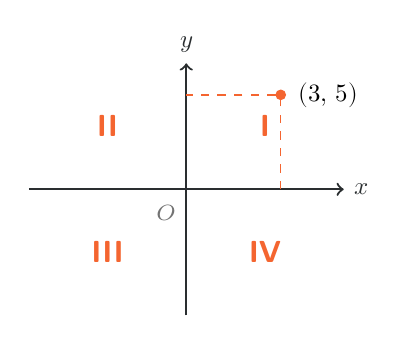
\begin{tikzpicture}
\draw[ink,line width=0.8pt,->] (-20mm,0) -- (20mm,0) node[right,font=\fontsize{9}{9}\selectfont] {$x$};
\draw[ink,line width=0.8pt,->] (0,-16mm) -- (0,16mm) node[above,font=\fontsize{9}{9}\selectfont] {$y$};
\node[font=\fontsize{8}{8}\selectfont,text=black!55] at (-2.5mm,-3mm) {$O$};

\node[font=\sffamily\bfseries\fontsize{11}{11}\selectfont,text=accent] at (10mm,8mm) {I};
\node[font=\sffamily\bfseries\fontsize{11}{11}\selectfont,text=accent] at (-10mm,8mm) {II};
\node[font=\sffamily\bfseries\fontsize{11}{11}\selectfont,text=accent] at (-10mm,-8mm) {III};
\node[font=\sffamily\bfseries\fontsize{11}{11}\selectfont,text=accent] at (10mm,-8mm) {IV};

\filldraw[accent] (12mm,12mm) circle (0.6mm);
\node[font=\fontsize{9}{9}\selectfont,anchor=west] at (13mm,12mm) {$(3,\,5)$};
\draw[accent,dashed,line width=0.5pt] (12mm,0) -- (12mm,12mm) -- (0,12mm);
\end{tikzpicture}
\end{textblock*}

\begin{textblock*}{50mm}(128mm,54mm)
{\fontsize{10.5}{14}\selectfont
\begin{tabular}{|>{\centering\arraybackslash}p{13mm}|>{\centering\arraybackslash}p{13mm}|>{\centering\arraybackslash}p{13mm}|}
\hline
\rowcolor{accent}
{\color{white}\textbf{Chorak}} & {\color{white}\textbf{$x$}} & {\color{white}\textbf{$y$}} \\ \hline
I & $+$ & $+$ \\ \hline
II & $-$ & $+$ \\ \hline
III & $-$ & $-$ \\ \hline
IV & $+$ & $-$ \\ \hline
\end{tabular}}
\end{textblock*}

% ================= CARD 2: y = kx + b (y: 99-154) =================
\cardbg{16}{99}{178}{55}
\pill{26}{102}{$y=kx+b$}

\begin{textblock*}{158mm}(70mm,120mm)
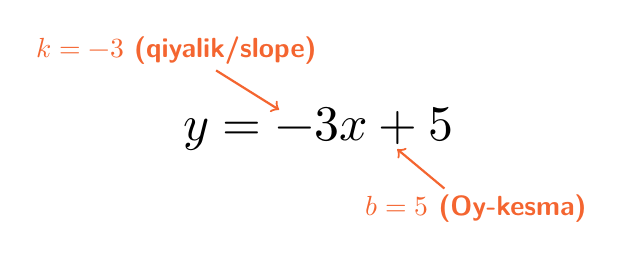
\begin{tikzpicture}
\node[font=\fontsize{18}{18}\selectfont] (eq) at (0,0) {$y=-3x+5$};
\node[font=\sffamily\bfseries\fontsize{10}{10}\selectfont,text=accent] at (-18mm,10mm) {$k=-3$ (qiyalik/slope)};
\node[font=\sffamily\bfseries\fontsize{10}{10}\selectfont,text=accent] at (20mm,-10mm) {$b=5$ (Oy-kesma)};
\draw[accent,->,line width=0.8pt] (-13mm,7.5mm) -- (-5mm,2.5mm);
\draw[accent,->,line width=0.8pt] (16mm,-7.5mm) -- (10mm,-2.5mm);
\end{tikzpicture}
\end{textblock*}

\begin{textblock*}{158mm}(26mm,147mm)
{\fontsize{9}{11}\selectfont\color{black!55}\itshape SAT'da $k$ o'rniga $m$ harfi va "slope" so'zi ishlatiladi: $y=mx+b$. $k=m$ -- faqat nom boshqa.}
\end{textblock*}

% ================= CARD 3: f(x) yozuvi (y: 160-265) =================
\cardbg{16}{160}{178}{105}
\pill{26}{163}{$f(x)$ yozuvi}

\begin{textblock*}{158mm}(26mm,177mm)
{\fontsize{11}{14}\selectfont\color{ink}
$f(x)$ -- bu shunchaki $y$ ning boshqa nomi. $x$ o'rniga son qo'yib, ifodani hisoblang:}
\end{textblock*}

\begin{textblock*}{158mm}(26mm,190mm)
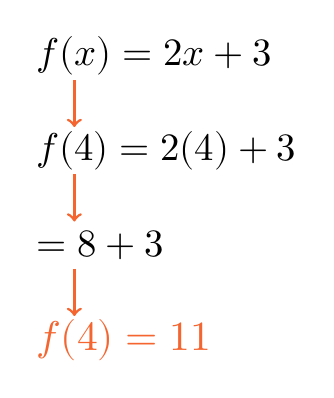
\begin{tikzpicture}[every node/.style={font=\fontsize{14}{14}\selectfont}]
\node[anchor=west] (a0) at (0,0) {$f(x)=2x+3$};
\node[anchor=west] (a1) at (0,-12mm) {$f(4)=2(4)+3$};
\node[anchor=west] (a2) at (0,-24mm) {$=8+3$};
\node[anchor=west,font=\sffamily\bfseries\fontsize{15}{15}\selectfont,text=accent] (a3) at (0,-36mm) {$f(4)=11$};
\foreach \y in {-3,-15,-27}{
  \draw[accent,->,line width=1pt] (6mm,\y mm) -- (6mm,\y mm -6mm);
}
\end{tikzpicture}
\end{textblock*}

\begin{textblock*}{158mm}(26mm,243mm)
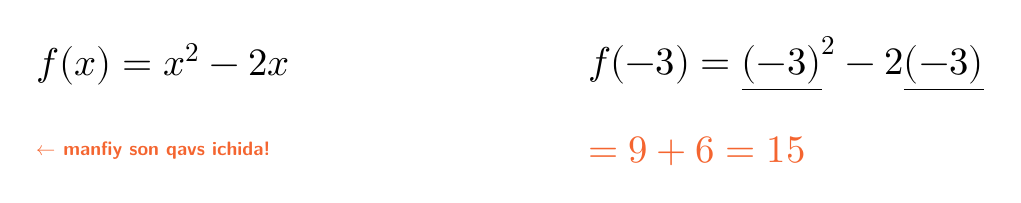
\begin{tikzpicture}[every node/.style={font=\fontsize{14}{14}\selectfont}]
\node[anchor=west] (b0) at (0,0) {$f(x)=x^2-2x$};
\node[anchor=west] (b1) at (70mm,0) {$f(-3)=\underline{(-3)}^2-2\underline{(-3)}$};
\node[anchor=west,font=\sffamily\bfseries\fontsize{14}{14}\selectfont,text=accent] (b2) at (70mm,-11mm) {$=9+6=15$};
\node[anchor=west,font=\sffamily\bfseries\scriptsize,text=accent] at (0,-11mm) {$\leftarrow$ manfiy son qavs ichida!};
\end{tikzpicture}
\end{textblock*}

\end{document}
